% !TeX root = 00_paper_entrypoint.tex

\section{Introduction}
Graphs allow flexible analyses of relationships among data objects. Thus, graph data management systems play an increasing role in present data analytics. Graphs have been already used as a fundamental data structure to represent data within different contexts such as corporate data \cite{success,Park2016355}, social networks \cite{xie,BrodkaK14} and linked data \cite{Vasilyeva13}.
Despite an increasing number of applications, a general operator that aggregates a single graph in a roll-up fashion is still missing. %partitions which the aforementioned vertices represent.
 The operation of adding structural aggregations to an existing graph is called \textit{graph nesting}.
A respective operator shall not only create a new graph of \textit{nested vertices} and \textit{nested edges}, each containing subgraphs of the original input graph, but also preserve the vertices and edges that are not affected by the actual operation. Further on, the operator must ensure that the nested elements can be freely unnested such that the original graph may be obtained back again. Vertices or edges of the original graph will be called \textit{members} of a nested vertex or edge, if they appear in its underlying subgraph.

\begin{figure}[!t]
  \begin{minipage}[!t]{0.5\textwidth}
    \centering
    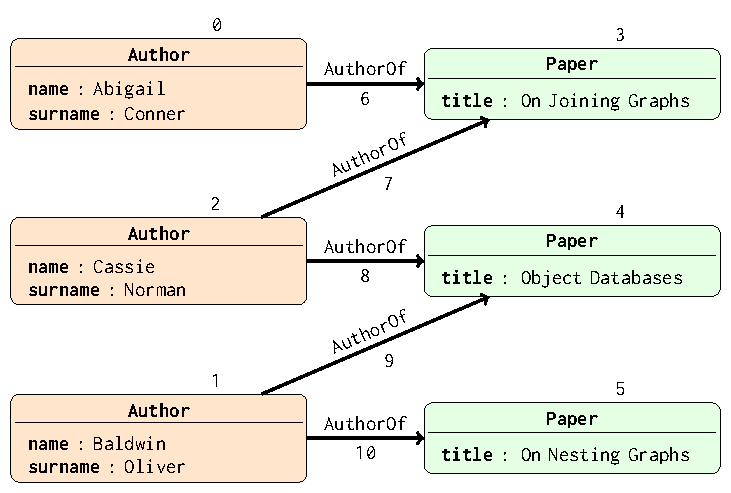
\includegraphics[width=.8\textwidth]{images/nesting/patterns/04bibliography.pdf}
    \subcaption{Input bibliographical graph represented as a Property Graph.}
    \label{fig:inputbibex2}
  \end{minipage}
  \medskip

  \begin{minipage}[!t]{0.5\textwidth}
    \centering
    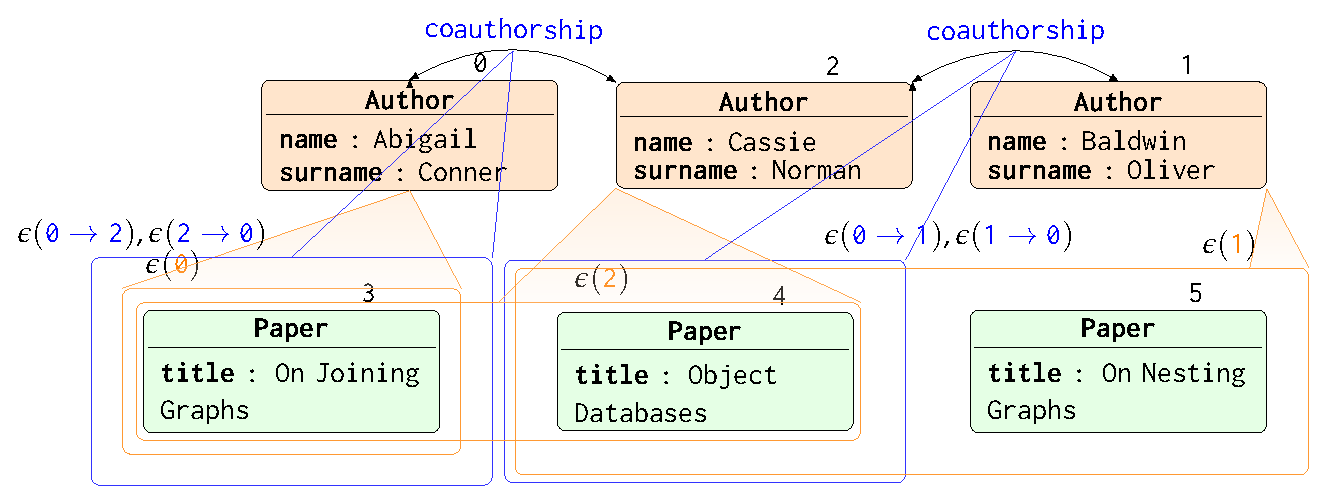
\includegraphics[width=\textwidth]{images/nesting/patterns/042nested.pdf}
    \subcaption{Nested required result: given two \texttt{Author}s $\color{orange}a$ and $\color{orange}a'$, there exist two  \texttt{coauthorship} edges, $\color{blue}a\to a'$ and $\color{blue}a'\to a$ if and only if they share some authored paper contained respectively in $\epsilon({\color{blue}a\to a'})$ and $\epsilon({\color{blue}a'\to a})$. Moreover, each author $\color{orange}a$ is associated to the set of his authored papers $\epsilon({\color{orange}a})$. }
    \label{fig:outputnested}
  \end{minipage}
\caption{Nesting a bibliographic graph: the provenance information is nested within the original node. }
\label{fig:bibex2}
\end{figure}

\begin{ex}[label=ex1]
Figure \ref{fig:inputbibex2} represents a bibliographic graph with (at least) \textsc{Author}s and \textsc{Paper}s as vertices and \textsc{authorOf} relationships as edges, which connect authors to papers they have authored. With the graph nesting operator, we want to ``roll up'' the graph into a coauthorship graph (Figure \ref{fig:outputnested}):  each \textsc{Author} will be connected by a \textsc{coAuthor} edge with another \textsc{Author}(2) if they have published at least one paper in common.
More precisely, each resulting \textsc{Author}(2) vertex shall contain authored papers as vertices and each \textsc{coAuthor} edge shall contain all the coauthored papers with regard to source and target \textsc{Author}s. However, we want to exclude \textsc{coAuthor} hooks over the same vertex.
\end{ex}

In a resulting nested graph, edges connecting nested vertices express that members of the nested vertices are connected by an edge or, more generally, by a path in the original graph.
In contrast to this general approach, current literature distinguishes between \textit{vertex summarization} and \textit{path summarization}. Thus, it is not possible to define a single query evaluating both kinds of patterns at the same time. Before outlining our proposed algorithmic solution, let's have a look on these existing approaches:

The \textit{vertex summarization} strategies group vertices in the manner of the relational \texttt{GROUP BY} operation and aggregate edges accordingly \cite{JunghannsPR17}. In this class of operations, summarized edges can only be formed by edges that directly connect members of summarized vertices in the original graph. In other words, these approaches cannot freely nest edges: for example, it is not possible to aggregate paths. Since most of vertex summarization techniques are based on graph partitioning, they further provide no support for nested vertices and edges with overlapping members \cite{yin,Tian20085,jakawat}.
Exceptions are HEIDS \cite{ChengJQ16} and Graph Cube \cite{Zhao11}, which perform graph summarizations of one single graph over a collection of non pairwise disjoint subgraphs. However, the union of these underlying subgraphs must be equivalent to the original graph, i.e., it is not possible to take vertices and edges of the original graph over to the summarized graph or to represent outliers that belong to no group.

%To overcome to this graph operation limitation, this thesis proposes the \textbf{graph nesting} operator, thus providing a general graph summarization technique.
%A straightforward implementation  proves to be inefficient, because the visit of such graph collections of size $k$ (to be nested within the graph operand) implies to perform, in the worst case scenario, $|g|^k$ visits of the graph operand $g$: this results into an exponential algorithm, because the size of $k$ may vary, while $|g|$ is fixed. This implies that the graph must be always visited more than once, even if this may not be required. Even though this general operator proves to be inefficient in practice, it allows to detect a broader class of problems and of optimizable algorithms.
%In order to reduce the graph visiting cost from $|g|^k$ to $O(|g|)$, we could use a graph traversal approach: instead of pre-computing $k$ subgraphs of $g$ that are going to be later on used to nest $g$, we can directly perform the graph nesting while visiting the graph, thus allowing  not to perform additional costs for comparing the resulting graphs in a later step. The following example shows how such queries can be efficiently formulated and implemented.
By contrast, \textit{path summarization} techniques allow the aggregation of multiple paths among pairs of source and target vertices that share the same properties.
%At the time of the writing, such approaches can be performed only over (graph) query languages.
Currently, approaches to path summarization can only be found within graph query languages.
%The problem with both path and vertex summarizations is that no general class of either source and target vertices can be used as an outcome of a previous community detection \cite{xie,berlingerio11} or data cleaning and alignment phase \cite{ALIEH17} without rewriting the previously extracted data into an explicit query, thus requiring an additional pre-processing step and thus making such approach not as flexible as required by data integration scenarios. %%initial query each time after different vertex data is extracted, thus not allowing to use such query definition for general data integration scenarios.
%This problem is also reflected by 
These languages also support vertex summarization, but no combination of both approaches in a single step.
%This constraint thwarts the advantages of performing vertex and path summarizations concurrently:
Cypher, the query language of the productive graph database Neo4j, can perform distinct aggregations only within distinct \texttt{MATCH} clauses. SPARQL, the standard query language of the resource description framework (RDF), requires to combine vertex and path aggregation with a \texttt{UNION} operator, i.e., the same input graph must be visited twice.
%As a result, the query plan optimizers of such query languages do not allow to avoid to visit one same graph more than once whether possible.

This paper shows that such query language limitations can be reduced by using a graph nesting operator, which performs both vertex and path summarization queries concurrently with only a single visit of the input graph. %The following example provides an example of how such query can be formulated and performed. --> Old example
We propose graph patterns to declare graph nesting operations and propose algorithmic optimizations as well as a specific physical model for efficient execution.
	
\begin{figure}[!t]
	\centering
	\begin{minipage}[!t]{0.5\textwidth}
		\centering
		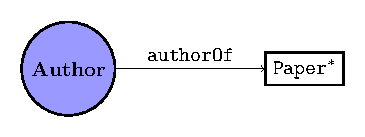
\includegraphics[width=.6\textwidth]{images/nesting/patterns/00_vertex_pattern.pdf}
		\subcaption{Vertex summarization pattern ($V$). Author is the vertex grouping reference $\gamma_V$.}
		\label{fig:vertexPat}
	\end{minipage} \begin{minipage}[!t]{0.4\textwidth}
		\centering
		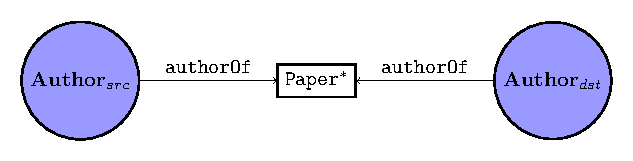
\includegraphics[width=1\textwidth]{images/nesting/patterns/00_path_pattern.pdf}
		\subcaption{Path summarization pattern ($E$). Author$_{src}$ and Author$_{dst}$ are respectively edge grouping references $\gamma_E^{src}$ and $\gamma_E^{dst}$.}
		\label{fig:pathPat}
	\end{minipage}
  \caption{Vertex and Path summarization patterns for the query expressed in the running example. Vertex and edge grouping references are marked by a light blue circled node. As we can see, the vertex grouping reference depicts the same property expressed by edge grouping references.}
\label{fig:patterns}
\end{figure}


\begin{ex}[label=ex2,continues=ex1]
	Figure \ref{fig:patterns} shows summarization patterns to describe the vertex ($V$) and path ($E$) nestings of our bibliographic network example: the former will create a nested \textsc{Author}(2) vertex and the latter will create a \textsc{coAuthor} nested edge. Given that $V$ appears twice in $E$, we may also pre-istantiate the pattern $V$ by visiting $E$ once. The two patterns have different key roles: while the vertex summarization retrieves all the \textsc{Paper}s that one \textsc{Author} has published and nest them within one single matched \textsc{Author}, the path summarization nests all the \textsc{Paper}s authored by two different \textsc{Author}s as members of a newly created nested edge connecting the two previously nested vertices. %This construction implies that a join between the two paths must be carried out.
	We can express this nesting requirement within vertex and path summarization patterns by electing both  \textsc{Author} in $V$ as a \textbf{vertex grouping reference} $\gamma_V$, and the two distinct \textsc{Author}s in $E$ (acting as the nested edge's source and targets) respectively as \textbf{edge grouping references} $\gamma_E^{src}$ and $\gamma_E^{dst}$. In particular, the two latter vertices must both match
	%For each vertex pattern we're going to elect one vertex as a \textbf{vertex grouping reference} ($\gamma_V$), in which we're going to nest the matched vertices and edges  during the graph traversal. Similarly, each edge path summarization pattern is going to elect a source ($\gamma_E^{src}$) and a target ($\gamma_E^{dst}$) vertex, which are going to be called \textbf{edge grouping references}: such vertces must both coincide 
	with the vertex grouping references, so that the newly generated edge will have as source and target the previously vertex-nested elements. In particular, this paper focuses on $E$ where $\gamma_E^{src}$  and $\gamma_E^{dst}$ are separated by a two-edge (hop) distance.
	
	
	We solve this problem by visiting the graph only once: %by visiting the graph starting from the vertices:
	If the current vertex is a \textsc{Paper}, traverse backwards all the \textsc{authorOf} edges, thus reaching all of its \textsc{Author}s ($\gamma_E^{src}$ and $\gamma_E^{dst}$), that are going to be \textsc{coAuthor}s for at least the current paper. Instead of associating the nesting content at the end of the graph visiting process, I can incrementally define the subgraph to be nested by using a separated nesting index: by visiting the two distinct \textsc{Author} vertices adjacent to the current \textsc{Paper}, the latter one shall be contained in both final \textsc{Author}(2) vertices, thus allowing the definition of a  \textsc{coAuthor} edge. %%The remaining types of vertices and edges %All the other vertices and edges
	%%may be discarded. %as a starting point for the graph visiting process
	By doing this, only the edges are visited twice, but the vertices are visited only once. These patterns allow to reach the optimal solution.
	
	%This pattern comparison remarks that, in order to reduce the graph time visit, we must start from visiting the \texttt{Paper}, which is shared among the two distinct patterns, and then keep going with the graph visit by exploring the source and target vertices. 
\end{ex}

%There might be other possible patterns that can be optimized, but we're going to focus just on vertex and path summarization patterns where edge grouping references are connected to each other at a 2 edge step distance (Section \ref{sec:THOSPA}). We're also going to show how such optimizations can be detected beforehand by looking at the pattern representation.


In the remainder of this paper, we will show that our algorithmic approaches reduce the time complexity of the visiting and nesting problem. Further on, our optimized data structure requires less indexing time than our competitors. This is achieved by the following contributions:

\begin{itemize}
	\item We propose a \textbf{Nested Graph Data Model} that is capable to implement the aforementioned solution of our example scenario. We use an optimized physical model that differs from the logical one (Section \ref{sec:model}).

	\item We provide  a general definition of a \textbf{Graph Nesting Operator} which combines vertex and path summarization approaches to nesting graphs (Section \ref{sec:nestingdef}).
	\item We introduce the  \textbf{\textsc{{Two HOp Separated Patterns}} (THoSP)} algorithm for graph nesting (Section \ref{sec:THOSPA}). We present the results of an experimental evaluation that compare it to alternative implementations using graph (SPARQL, Cypher), relational (SQL) and document oriented (AQL) query languages: our solution outperforms all competitors by at least one order of magnitude in average with regard to the sum of both indexing and query evaluation time (Section \ref{sec:nestexpeval}).

%  the aforementioned solutions evaluated on such databases with their respective query languages . Consequently, our data model also proved to be crucial in providing an enhanced implementation of the specific graph nesting task.
	%\item A general strategy on how to extend the THoSP algorithm for patterns having vertex and edge grouping references is provided (Section \ref{sec:optimizableClass}).
	%%\item By extending the concept of binary predicates into edges, Edge Joins are introduced as a preliminary step towards the definition of Graph Nesting (Chapter \ref{cha:nesting}).
\end{itemize}

The source code for THoSP is provided at \texttt{\color{red}[Link removed for double-blind review]}.
